\documentclass{article}

\usepackage{fancyhdr}
\usepackage{ragged2e}
\usepackage{graphicx}
\usepackage{caption}
\usepackage{geometry}
\usepackage{amsmath}
\usepackage{rotating}

\usepackage{listings}
\usepackage{color}

\definecolor{dkgreen}{rgb}{0,0.6,0}
\definecolor{gray}{rgb}{0.5,0.5,0.5}
\definecolor{mauve}{rgb}{0.58,0,0.82}

\lstset{frame=tb,
  language=Java,
  aboveskip=3mm,
  belowskip=3mm,
  showstringspaces=false,
  columns=flexible,
  basicstyle={\small\ttfamily},
  numbers=none,
  numberstyle=\tiny\color{gray},
  keywordstyle=\color{blue},
  commentstyle=\color{dkgreen},
  stringstyle=\color{mauve},
  breaklines=true,
  breakatwhitespace=true,
  tabsize=4
}

\setcounter{secnumdepth}{1}

\usepackage{chngcntr}
\counterwithin{figure}{section}

\renewcommand*{\thepage}{C\arabic{page}}

\pagestyle{fancy}
\lhead{ACME Robotics}
\chead{\#8367}
\rhead{\ifcontents Contents \else Week \thesection \fi}

\newif\ifcontents
\contentstrue

\makeatletter
\renewcommand{\@seccntformat}[1]{}
\makeatother

\begin{document}\contentsfalse

\subsection{Finish Designing the team marker}
%! CAD the team marker.
Shawn and Ben worked on developing a new team marker that was an anvil. Ben took the old anvil hat CAD from last year and derived the file and re-scaled it to fit in the proper dimensions. Ben then added a hook and for the mechanism and engraved the top of the anvil with the team marker. They then rendered the model. At the next meeting, they further developed the mechanism.

\subsection{Complete Sorter and Intake CAD}
%! Editing the Sorter and attachments.
Ashlin and Aidan worked on finalizing the attachment of the sorter to the intake and the rest of the robot as shown in \ref{fig:Intake CAD}. They put the sorter at a 45 degree angle to so that the objects would naturally go into the sorter and out into the cartridges easily because of the steep angle. Because of this they needed to edit the size of the cartridges so that the cartridges would have enough room to be raised up. They also attached a servo to the bottom of the sorter that it would be what rotates the sorter in either direction depending on if the item is a ball or cube.

\begin{figure}
    \centering
    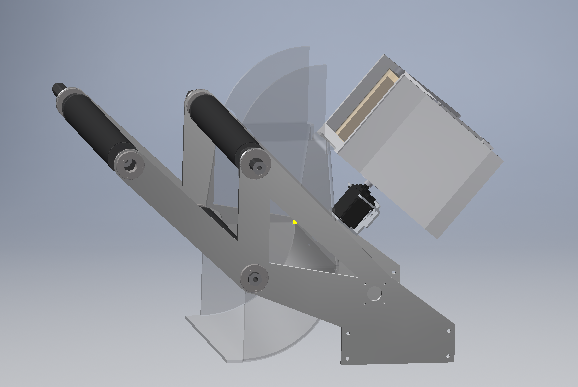
\includegraphics[width=.6 \textwidth]{07_10-15/images/IntakeCAD.png}
    \caption{Sorter and Intake CAD}
    \label{fig:Intake CAD}
\end{figure}

\subsection{Testing Rev Linear Slide Kit}
%! Build the linear slide system. 
Recently, the team received the Rev linear motion kits they ordered. To see how exactly the kit went together and see it would be mounted on the robot; Jon put some of the kit together. Jon made several segments, measured, and calculated the exact amount of 15 mm extrusion would be needed for the robot. This gave the team a better idea of how it would be assembled on the robot and a basis for CAD.
\subsection{CNC Milled Drive-Train }
%! Cut Drive-Train Plates.
Oren, Ashlin, and Kelly worked with the Nu wood-shop teacher, to use their new CNC Laguna to cut out the 1/8 inch aluminum plates that make up the entirety of the drive-train. They had learn how to do auto tool changes and setting the X,Y and Z axis on the new tool as to allow them the most accurate product in the end
\end{document}

